\documentclass[a4paper, titlepage]{article}

\setlength{\parindent}{0em}
\setlength{\parskip}{1em}

\usepackage[a4paper, portrait, margin=1in]{geometry}

\usepackage{graphicx}

\title{MMEA Developer's Guide}
\author{Lukas Turcani}
\begin{document}
\maketitle
\tableofcontents
\pagebreak

\section{Document description}
The role of this document is to provide an overview of the MMEA program and its constituent code. It is not intended to provide a detailed account of the software or its features. Any changes to the software should adhere to the descriptions and guidelines presented here, as it is mostly an account of the design rather than specific functions, methods, classes, etc. As a result, this document should be relatively resilient to changes in the code.
       
\section{Program overview}

\begin{figure}[h]
	\centering
	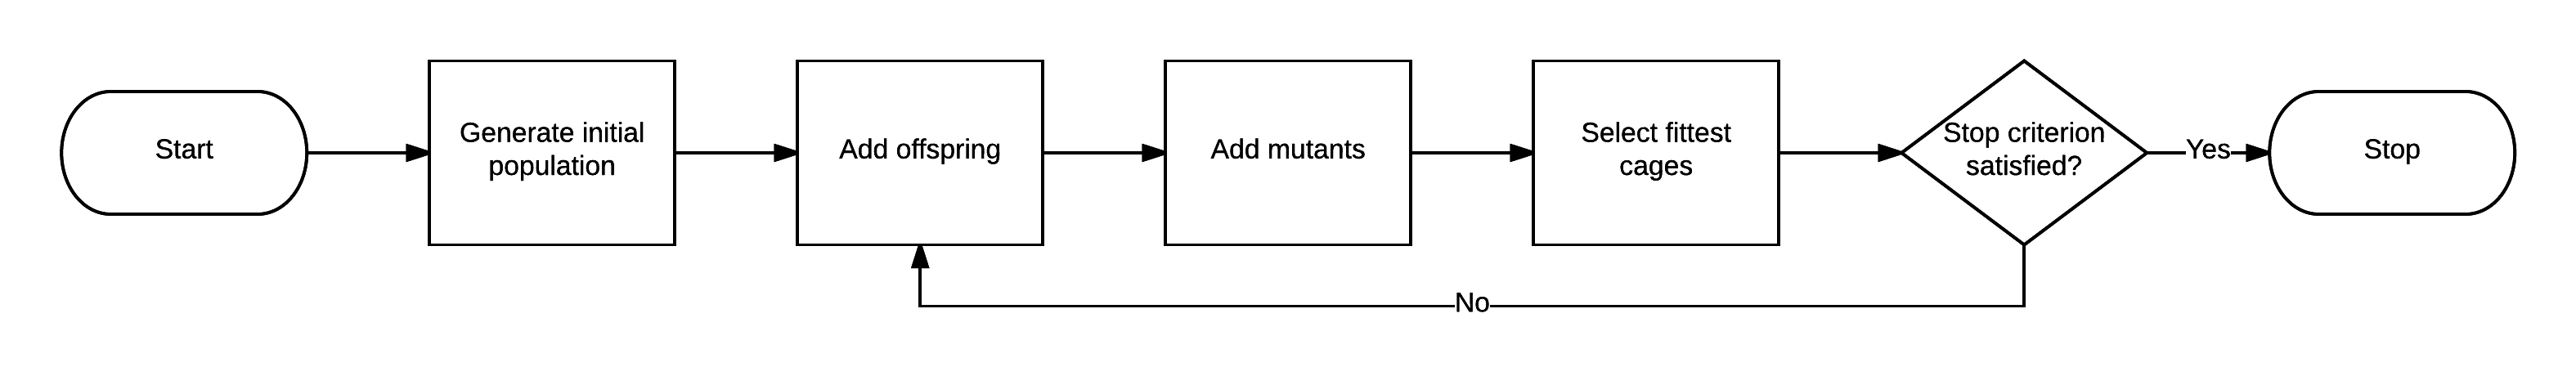
\includegraphics[width=\textwidth]{./figures/program_overview/MMEA_flow_horizontal.png}
	\caption{Flow diagram of MMEA execution.}
	\label{flow_diagram}
\end{figure}

MMEA is a genetic algorithm.

\section{Design goals}

\begin{enumerate}
	\item Extensibility and maintainability.
	\item Speed.
\end{enumerate}

\section{Class overview}

\section{Style guide}

\section{Extending MMEA}

\end{document}